% !TeX spellcheck = fr_FR

% TODO: Replace scan images with clean text where possible

\documentclass[a4paper, 10pt]{report}

\usepackage[french]{babel}
\usepackage[T1]{fontenc}

\usepackage{amsmath, amssymb, amsfonts}

\usepackage{hyperref}
\usepackage{geometry}

\usepackage{xcolor}
\usepackage{graphicx}

\usepackage{fancyhdr}
\usepackage{lastpage}

\usepackage{enumitem}

\geometry{
	a4paper,
	left=25mm,
	right=25mm,
	top=35mm,
	bottom=25mm,
	headsep=5mm,
	headheight=20mm,
}

\definecolor{solution}{HTML}{E5E4E2}
\providecommand{\abs}[1]{\lvert#1\rvert}
\providecommand{\norm}[1]{\lVert#1\rVert}
\DeclareMathOperator{\card}{card}

\makeatletter
\renewcommand*\env@matrix[1][*\c@MaxMatrixCols c]{%
	\hskip -\arraycolsep
	\let\@ifnextchar\new@ifnextchar
	\array{#1}}
\makeatother

\begin{document}
	
	\renewcommand{\headrule}{%
		\vspace{-4pt}\hrulefill
		\raisebox{-6.8pt}{\ 
\includegraphics[height=5mm]{../../icon.png}}
		\hrulefill
	}	
	\pagestyle{fancy}
	\fancyhf{}
	
	\fancyhead[L]{\small \slshape Automne 2024}
	\fancyhead[C]{\Large \bfseries Algèbre I - Série 07}
	\fancyhead[R]{\small Buff Mathias}
	\fancyfoot[L]{
		\small Source files available at:
		\href{https://github.com/MathiasBuff/bsc-math}
		{github.com/MathiasBuff/bsc-math}
	}
	\fancyfoot[R]{
		\small Page \thepage
		\hspace{1pt} /
		\pageref*{LastPage}
	}
	

	\noindent
	\textbf{Exercice 1.} (Matrice de rotation)\\
	Soit $\theta \in \mathbb{R}$. On note $\rho_\theta$ l'application
	linéaire qui à un vecteur $\vec{v}$ de $\mathbb{R}^2$ associe sa
	rotation par un angle trigonométrique $\theta$.\\
	On note aussi $\mathrm{Pr}_\theta$ l'application linéaire qui à un vecteur $\vec{v}$ associe sa projection orthogonale sur la droite $d_\theta$ (la droite du plan passant par l'origine et formant un
	angle trigonométrique $\theta$ avec le vecteur $e_1 = (1, 0)$).
	
	\begin{enumerate}[label=\arabic*.]
		\item Calculer directement les matrices associées à ces
		applications linéaires, $M(\rho_\theta)$ et
		$M(\mathrm{Pr}_\theta)$, dans la base canonique de $\mathbb{R}^2$
		%
		\item Montrer que $M(\rho_{\theta + \theta'})
			= M(\rho_\theta)M(\rho_\theta')$
		%
		\item En déduire que l'application $\rho_\theta$ est inversible
		et calculer son inverse.\\
		L'application $\mathrm{Pr}_\theta$ est-elle inversible ?
	\end{enumerate}
	
	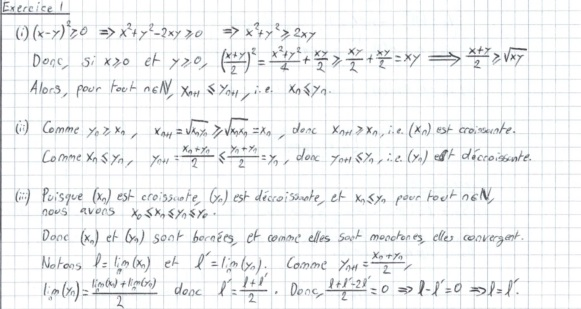
\includegraphics{ex01.jpg}
	
	\newpage
	
	\fancyhf{}
	\renewcommand{\headrule}
	{\rule{\textwidth}{0pt}}
	\fancyfoot[R]{
		\small Page \thepage
		\hspace{1pt} /
		\pageref*{LastPage}
	}
	
	\noindent
	\textbf{Exercice 2.} (Endomorphisme de dérivation)\\
	Considérons l'espace $\mathcal{P}_n$ des polynômes de degré au plus
	$n$ en une variable à coefficients réels\\
	(noté aussi $\mathbb{R}_n[x]$). Soit $D$ l'application de dérivation,
	qui à un polynôme associe son polynôme dérivé.
	
	\begin{enumerate}[label=\arabic*.]
		\item Calculer la matrice $M(D)$ associée à l'endomorphisme $D$
		dans la base canonique de $\mathcal{P}_n$,
		$\{1, x, x^2, \dotsc, x^n\}$
		%
		\item Calculer $\mathrm{Im}(D)$ et $\mathrm{Ker}(D)$, puis
		vérifier le théorème du rang.\\
		\textit{\textbf{Remarque :} Comparer à l'exemple de l'endomorphisme
			D de dérivation opérant dans l'espace $\mathcal{Pol}$ de
			polynômes de tout degré, vu au cours (§1, Chap. III).}
	\end{enumerate}
	
	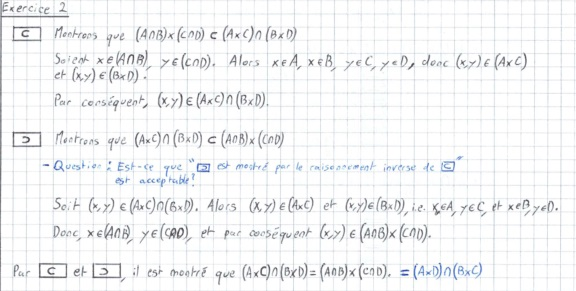
\includegraphics{ex02.jpg}
		
	\vspace{5mm}
	\noindent
	\textbf{Exercice 3.} (Un changement de base)\\
	\textit{\textbf{Rappel :} On note $M_{\mathcal{C,B}}(f)$ la matrice
		de l'application linéaire $f: E \to F$, où $\mathcal{B}$ est la
		base de départ (pour l'espace vectoriel E) et $\mathcal{C}$ est
		la base d'arrivée (pour l'espace vectoriel F).}\\
		
	\noindent	
	Soit $\mathcal{B}$ la base canonique de $\mathbb{R}^3$ et
	$\mathcal{C} = 
		\left\{
		\begin{pmatrix}	1\\2\\-1 \end{pmatrix},
		\begin{pmatrix}	0\\1\\2 \end{pmatrix},
		\begin{pmatrix}	1\\1\\-1 \end{pmatrix}
		\right\}$.\\
	
	\noindent
	Montrer que $\mathcal{C}$ est bien une base de $\mathbb{R}^3$
	puis déterminer $M_{\mathcal{B,C}}(\mathrm{Id}_{\mathbb{R}^3})$
	et $M_{\mathcal{C,B}}(\mathrm{Id}_{\mathbb{R}^3})$. Vérifier que
	ces deux matrices sont bien inverses l'une de l'autre.
		
	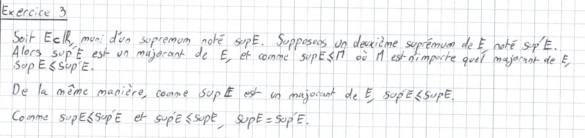
\includegraphics{ex03.jpg}
	
	\newpage
	
	\noindent
	\textbf{Exercice 4.} (L'image d'un vecteur)\\
	Soient $\mathcal{B} = \{1, x, x^2, x^3\}$ et
	$\mathcal{C} = \{1, 1 + x, 1 + x + x^2, 1 + x + x^2 + x^3\}$ deux
	bases de l'espace vectoriel $\mathcal{P}_3$. Considérons
	l'application linéaire
	\[\begin{aligned}
		f :&& \mathcal{P}_3 &\to \mathcal{P}_3\\
		&& p(x) &\mapsto p(x + 1)
	\end{aligned}\]
	\begin{enumerate}[label=\arabic*.]
		\item Pour le polynôme $p(x) = 1 + 2x + 4x^2 + 8x^3$, calculer
		$f(p)$ dans la base $\mathcal{B}$
		%
		\item Pour le même polynôme, calculer $f(p)$ dans la base
		$\mathcal{C}$
		%
		\item Calculer la matrice $M_{\mathcal{C,B}}(f)$
		%
		\item Utiliser la question précédente pour déduire $f(p)$ dans
		la base $\mathcal{C}$
	\end{enumerate}
	
	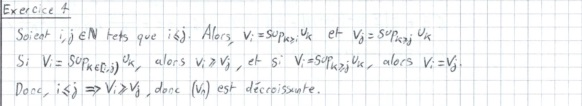
\includegraphics{ex04.jpg}
	
	\newpage
	
	\noindent
	\textbf{Exercice 5.} (Matrices de passage)\\
	Considérons les bases de $\mathbb{R}^2$
	\[
		\mathcal{B} = 
			\left\{
			\begin{pmatrix} 1\\1 \end{pmatrix},
			\begin{pmatrix} 1\\0 \end{pmatrix}
			\right\}
		\ \text{et}\ \mathcal{B'} =
			\left\{
			\begin{pmatrix} 0\\1 \end{pmatrix},
			\begin{pmatrix} 2\\1 \end{pmatrix}
			\right\}
	\]
	Trouver les matrices de passage $\mathcal{P_{B', B}}$ et
	$\mathcal{P_{B, B'}}$, puis vérifier que
	$\mathcal{P_{B', B}} \mathcal{P_{B, B'}} 
		= \mathrm{Id}_{\mathbb{R}^2}$
	
	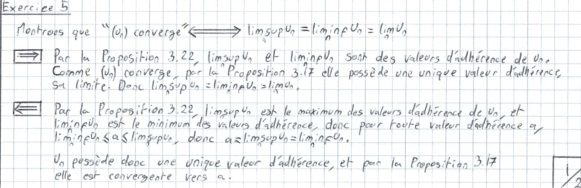
\includegraphics{ex05.jpg}
	
	\vspace{5mm}
	\noindent
	\textbf{Exercice 6.} (Rang, noyau et image d'une matrice)\\
	Déterminer le rang, le noyau et l'image de la matrice
	\[\begin{pmatrix}
		1 & 2 & 3 & 2\\
		4 & 8 & 2 & -2\\
		1 & 2 & 1 & 0
	\end{pmatrix}\]
	
	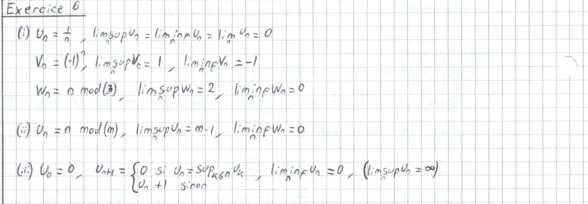
\includegraphics{ex06.jpg}
	
	
%	
%	\colorbox{solution}
%	{
%		\begin{minipage}{0.9\textwidth}
%			s
%		\end{minipage}
%	}
%	
%	\colorbox{solution}
%	{
%		\begin{minipage}{0.9\textwidth}
%			\begin{enumerate}[label=(\alph*)]
%				\item a
%			\end{enumerate}
%		\end{minipage}
%	}
	
\end{document}
